\frame
{
	\frametitle{Distributed Online Learning for Pattern Prediction}
	%\framesubtitle{Maritime Surveillance}
	%\framesubtitle{Proposed System Model}
	\begin{center}
		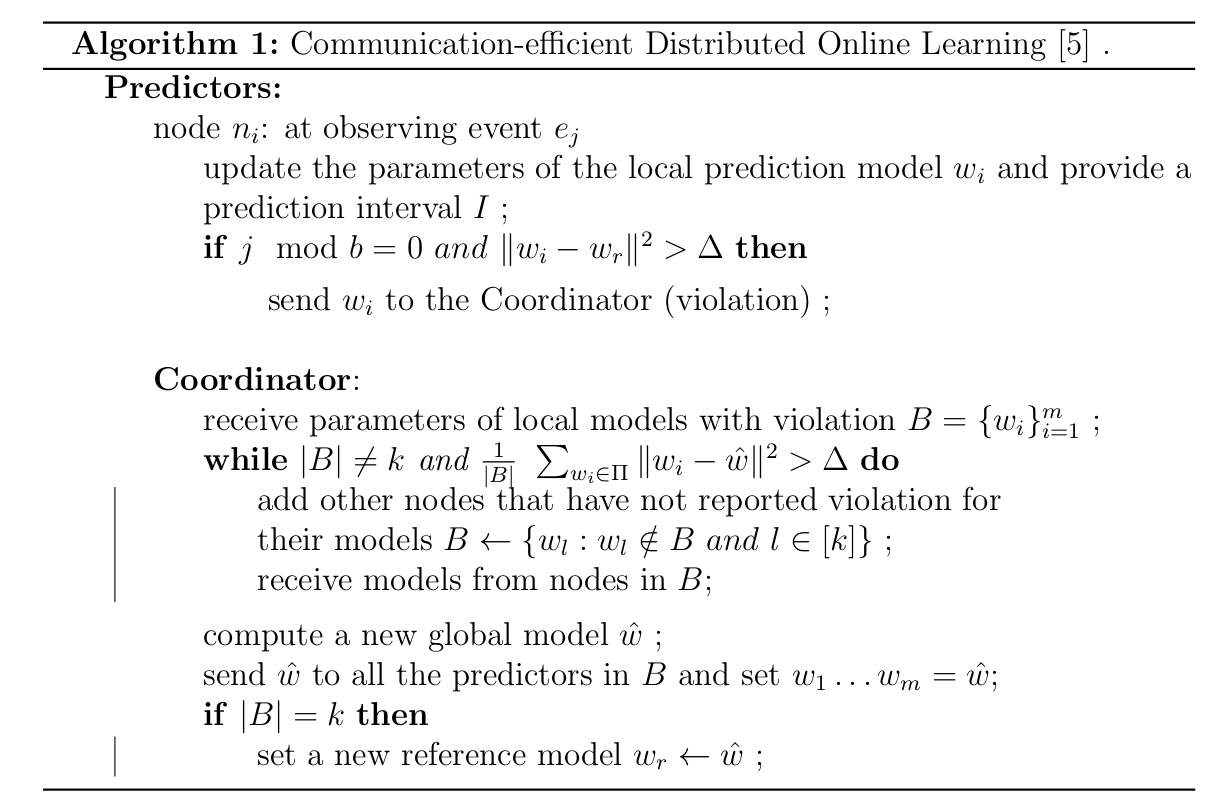
\includegraphics[width=\textwidth,left]{figures/new/dol.png}\\
.
	\end{center}
}


\frame
{
	\frametitle{ Communication-Efficient Distributed Online Prediction by Dynamic Model Synchronization  \citep{kamp2014communication}}
	\framesubtitle{}
	\begin{itemize}[]
		\item<1-> A protocol for distributed online prediction over multiple input data streams in a communication efficient manner.
		\item<1-> It allows to combine local models into a global model
	using a $synchronization$ $ operation$.
		\item<1-> The distributed learners exchange their local model with a central coordinator node periodically after observing a fixed number of data points (i.e., mini-batches) \citep{dekel2012optimal}.
		
		\item<1-> A dynamic synchronization scheme based on monitoring the local models variance from a global reference model ($\|f_i - r\|^2 \leq \bigtriangleup$).
		
		
%		dynamic synchronization scheme within which the learners communicate only if their local models diverge from a global reference point
	\end{itemize}
}

\frame
{
	\frametitle{Distributed Online Learning for Pattern Prediction}
		%\framesubtitle{Proposed Synchronization Operation}
	\begin{itemize}[]

	\item<1-> The
 $synchronization$ $ Operation$ for the global transition probability matrix $\hat{\Pi}$:
 \begin{equation*}
 \label{eq:dis_pi_estim}
 \hat{\pi}_{i,j} = \frac{\sum_{k \in K} n_{k,i,j}}{\sum_{k \in K} \sum_{l \in L} n_{k,i,l}}
 \end{equation*}

Where $n_{k,i,j}$ the number of transitions from state $i$ to state $j$ on node $k$.
	
\end{itemize}
}

\frame
{
	\frametitle{Distributed Online Learning for Pattern Prediction}
	%\framesubtitle{Proposed Synchronization Operation}
	\begin{itemize}[]
		
		\item<1->The divergence of the local models from the reference model $\|w_i - w_r\|^2$ is calculated by the sum of square difference between the local transition probability matrix $\Pi_i$ and the reference transition matrix $\Pi_r$:
		\begin{equation*}
		\label{eq:dis_pi_varinace}
		\|w_i - w_r\|^2=|\Pi_i - \Pi_r\|^2=\sum_{l,j} (\pi{i,l,j} -\pi{r,l,j})^2
		\end{equation*}
		
	\end{itemize}
}


\frame
{
	\frametitle{Distributed Online Learning for Pattern Prediction}
	\framesubtitle{Probabilistic Learning Guarantee}

		
		\begin{equation*}
		\begin{aligned}
		\label{eq:guarantee}
		\Pr\left( |\hat{\pi}_{i,j} - {p}_{i,j}| \geq c \right) \leq
		\frac{1}{k}\ \Pr\left( |\hat{p}_{i,j} - {p}_{i,j}| \geq c \right)
		\end{aligned}
		\end{equation*}
		
	
}